\documentclass[a4paper,12pt,fleqn,oneside]{scrartcl}
\usepackage[usenames,dvipsnames]{xcolor}
\usepackage[english]{babel}
\usepackage[utf8]{inputenc}
\usepackage[T1]{fontenc}
\usepackage[toc,page]{appendix}
\usepackage{floatflt}
\usepackage{lmodern}
\usepackage{amssymb}
\usepackage{amsmath}
\usepackage{enumerate}
\usepackage{fancyhdr}
\usepackage{pgfplots}
\usepackage{multicol}
\usepackage{tikz}
\usepackage[hidelinks]{hyperref}
\usepackage{listings}
\usepackage{mdframed}
\usepackage{tabularx}
\usepackage{booktabs}
\usepackage{pgfplots}
\usepackage{pgfplotstable}
\usepackage{float}
\usepackage{wrapfig}
\usepackage{blindtext}
\usepackage{etoolbox}
\usepackage{lastpage}
\usepackage{tocloft}
\usepackage{graphicx}
\usepackage{caption}
\usepackage{subcaption}
\usepackage[asymmetric,top=1.5in,bottom=1.5in,left=1.2in,right=1.2in]{geometry}
\usepackage[sectionbib]{natbib}

\usepackage{tgpagella}
% \usepackage{quattrocento}

\usetikzlibrary{shapes,arrows,calc,patterns,decorations.markings,shadows.blur}

\title{Saliency maps}
\author{Paul Bienkowski \\[0.2em] \scriptsize 2bienkow@informatik.uni-hamburg.de}
\date{\today}

\pagestyle{fancy}
\fancyhf{}
\fancyhead[L]{Seminar ``Brain Modelling'' 2014}
\fancyhead[R]{Saliency Maps}
%\setlength{\footskip}{2em}
%\setlength{\footrulewidth}{0.4pt}
\fancyfoot[L]{\small{}Paul Bienkowski}
\fancyfoot[R]{\small{}Page \thepage  \:of \pageref{LastPage}}

\newif\iffinal
\finaltrue

% \renewcommand{\arraystretch}{1.2}
% \renewcommand{\arraystretch}{1.5}
% \renewcommand{\familydefault}{\sfdefault}
\linespread{1.1}

\let\stdsection\section
% \renewcommand\section{\newpage\stdsection}
\setlength{\parindent}{0pt}
% \setlength{\parskip}{1.8ex}
\setlength{\parskip}{1.0ex}

\begin{document}

\begin{titlepage}
    \begin{center}

    \textsc{\Large Seminar 2014}\\[0.0cm]
    \textsc{\small ``Brain Modelling''}\\[0.0cm]
    \textsc{\small Universität Hamburg}
    \\[0.5cm]
    \textsc{\today}\\[0.5cm]

    % Title
    \rule{0.8\textwidth}{0.4pt}
    \\[0.4cm]
    {\huge \bfseries \textsc{Saliency Maps}}
    \\[0.0cm]
    \rule{0.8\textwidth}{0.4pt}\\[1.2cm]

    % Author and supervisor
    \begin{minipage}{0.4\textwidth}
        \begin{flushleft} \large
            Paul \textsc{Bienkowski}\\[-0.1cm]
            {\small Author}\\[-0.2cm]
            {\scriptsize \url{2bienkow@informatik.uni-hamburg.de}}
        \end{flushleft}
    \end{minipage}\begin{minipage}{0.4\textwidth}
        \begin{flushright} \large
            Cornelius \textsc{Weber}\\[-0.1cm]
            {\small Supervisor}\\[-0.2cm]
            {\scriptsize \url{weber@informatik.uni-hamburg.de}}
        \end{flushright}
    \end{minipage}

    \vfill

    \textsc{Abstract}\\[-0.0cm]
    \rule{0.8\textwidth}{0.4pt}\\[0.2cm]
    \end{center}

    \begin{minipage}{0.10\textwidth}\-\end{minipage}\begin{minipage}{0.8\textwidth}
    {\small 

        Visual attention modelling is a key to understanding how the human brain
        is able to focus on the important things to see. Such a model can be
        used in a wide field of technology, for instance in robotic systems,
        computer graphics or computer visition. In this paper I will explain the
        principles of the pre-attentive visual system, that is the part of the
        visual system that controls the focus of attention, and compare
        different modelling approaches with their neuro-biological counterparts
        inside the visual system. I will show that early models, such as the one
        by Itti and Koch from the year 2001, closely follow insights from
        neurobiological studies trying to imitate the brain as closely as
        possible, while the later ones, for example Perazzi from 2012, are only
        inspired by the visual system and divert from true modelling to achieve
        various effects. I will explain both models in detail, as well as the
        the effects achieved, and the real world applications they can be used
        for.

    }
    \end{minipage}

\end{titlepage}

\tableofcontents

\newpage
\section{Introduction}

\subsection{Motivation}

Visual attention describes the mechanisms in the human brain that mainly control
what we look at -- the steps and stages in the visual system that help control
eye movement, thus finding important features in a visual scene. It furthermore
filters the peripheral field of view for intense stimuli, thus reducing the
amount of visual data to be processed. Visual attention is crucial to recognise
our surroundings and an ongoing task. It even has evolutionary relevance since
fast and good visual detection are great advantages for both predator and prey.

Part of the fascination about the way the human brain perceives visual scenes and finds objects of interest is in the
speed and robustness it achieves doing so. By understanding the inner neuro-biological workings, we hope to achieve similar
results in artificial recognition technologies, which can be used in a wide field of applications, especially robotics,
surveillance or navigational aid.

However, visual attention approaches can be used in other contexts as well, being adjusted to the  needs of the context.
In computer graphics, object recognition and object boundary detection are frequent tasks that can be achieved by
similar means. In these cases, the neuro-biological findings are often used as a starting point in developing new methods.

There are many different approaches to explain and simulate the processes that make up visual attention. Most
explanations however first divide it up into bottom-up and top-down parts. The bottom-up approach deals solely with
image-based processing, not interpreting the objects in the visual scene but rather working mainly with localized
contrast and center-surround mechanisms, combining them into different maps that represent visual saliency. The top-down
approach is guided by the task at hand and much more complex, taking into account knowledge and intention of the
perceiving person.

In this paper I will compare different approaches explaining the neuro-biological visual  attention system with some
algorithms for different related use-cases. I will focus on bottom-up approaches, always keeping in mind how they
interact with the top-down parts in the visual system.

\subsection{Examples}

Figure~\ref{fig:examples} displays some examples for saliency maps generated from an input image (a). The grayscale
images (b) through (g) are saliency maps, in which white depicts high values of saliency, dark colors depict less
salient regions. It is very clear that there are many possible and different saliency maps that can be generated. The
first three (b), (c) and (d) are rather blurry, but their highest saliency values are distributed around the object of
interest. Algorithm (e) yields high saliency values on object boundaries, similar to an edge detection algorithm. The
last two (f) and (g) then highlight whole objects thay may be of interest, in these maps  it is still possible to find
details.

All these algorithms may be useful for a specific task. While the latter ones are more useful in object boundary
detection, the former are usually easier to compute and find points of interest for further analysis.

\begin{figure}[hbt]
    \centering
    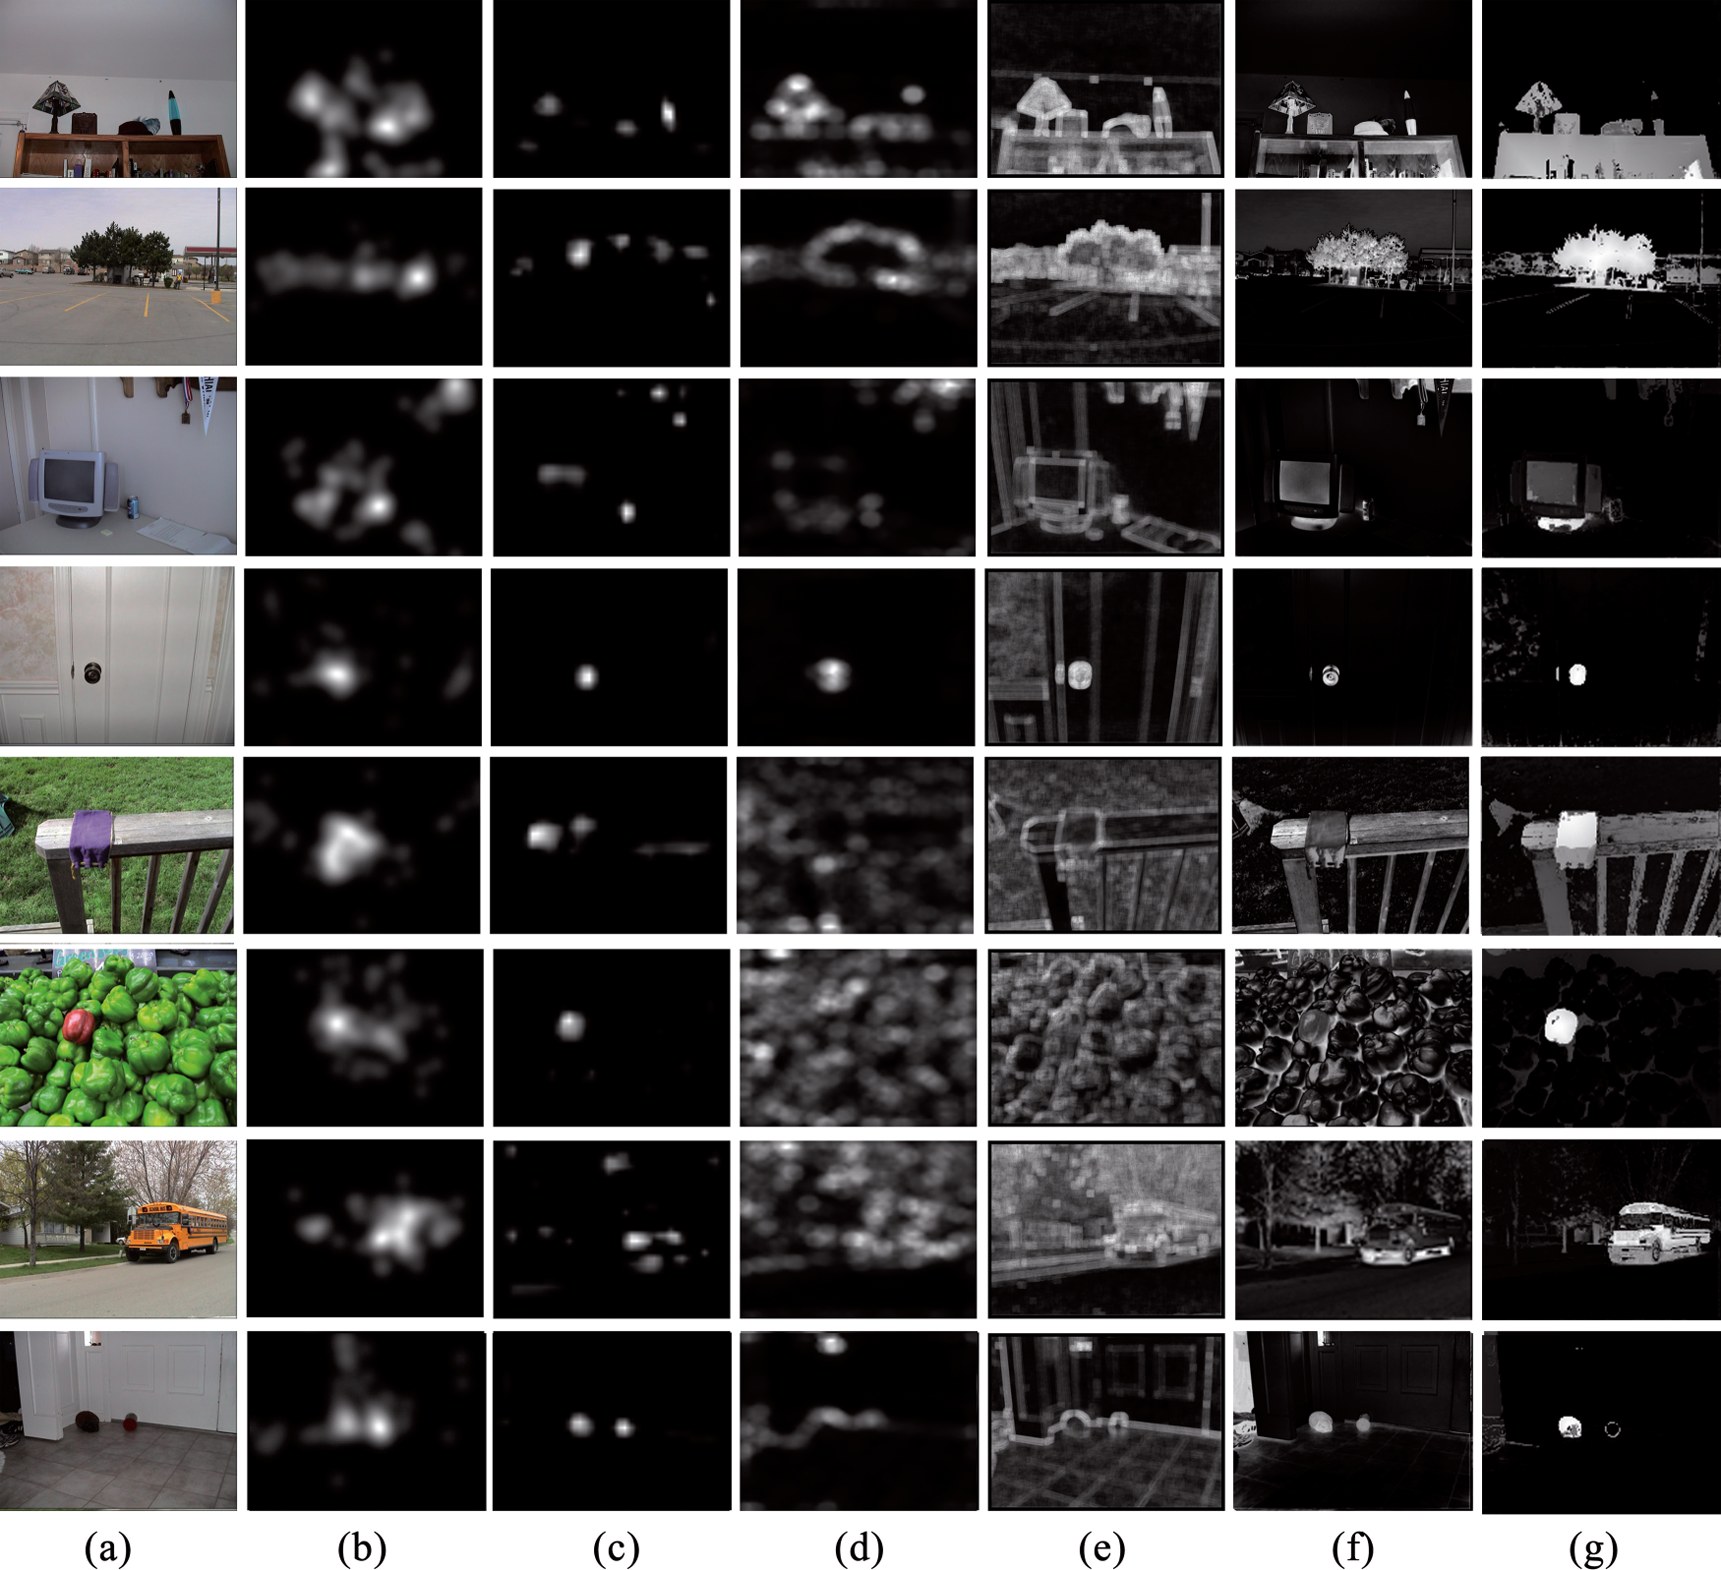
\includegraphics[scale=0.8]{examples.png}

    \caption[\url{http://opticalengineering.spiedigitallibrary.org/data/Journals/OPTICE/23430/057008_1_6.png}]{Different
    algorithms yield different maps -- for different applications. For reference, the columns corresponding to
    the subsequently presented algorithms are: Koch/Itti (b), Hou (c), Perazzi (g).}
    \label{fig:examples}
\end{figure}

% \textit{DISCUSSION} Using the Lab color space, an algorithm does not require to differenciate between
% brightness, hue, saturation etc. but can instead use one unified measure for 
% contrast calculations, the color distance.

\section{Methods}

In this section I will describe a few terms and methods that are used by almost any approach and where these methods can
be found inside the visual system, neuro-biologically modelled.

\subsection{A word about Contrast}

The concept of \textit{contrast} is being used quite often in the context of saliency detection. However, the definition
may vary between publications on this topic, depending on the data it is applied to and the effect to achieve.
\emph{Color intensity} contrast is a measure to describe the difference in color perception, either based solely on brightness (in
cases with grayscale pictures) or the perceived color variance.  To technically measure this color variance, an
appropriate color representation has to be used. The \textsc{Lab} color space describes a representation based on human
perception. It uses three components, the \textbf{L}ightness and two dimensions of  complementary color (\textbf{a},
\textbf{b}) and is designed to model the perceived color as realistically as possible. Calculating the Euclidean
distance between two colors in this space yields a reasonable contrast measure.

The reference value for the contrast calculation however can be obtained in different ways. Mainly, there is a
difference between global and local contrast. Some simple algorithms calculate the contrast-based saliency value based
on the color difference to the mean color of the whole scene. While this is an easy and simple approach, it is to argue
how accurate this models the human brain, which rather works mainly with center-surround cell linking, yielding a local
contrast measure. Either way, most algorithms normalize local contrast based on the image mean brightness, as the eye
does by adjusting the iris.

Furthermore, the contrast measure can be based not only on spatial color distribution, but also temporal change. While
the inner receptive fields of the retina, the fovea, have high spatial resolution, allowing us to perceive every detail,
the outer parts are instead connected to parts of the visual system with higher temporal resolution. In
these outer parts, contrast can also be determined in the temporal domain, so movements ``in the corner of the eye'' are
more likely to catch our attention and cause a saccade to detect the object.

\subsection{Blurring}

Blur filters are often used in saliency map algorithms. Their main goal is to calculate a mean color for a local patch
in order to remove detail from an image  by taking neighboured pixels into account. The filter adds the colors with a
weighted function based on their relative position. This is very easy to implement in a neural network, as it can be
done with a simple topographical perceptron  layer and only local connections.  This process can also be applied on
other (multidimensional) data for various effects.

An often used weight function for blurs is the Gaussian distribution, which yields a smoothed texture and can be
decomposited into multiple passes, one for each dimensions, resulting in a linear instead of polynomial runtime. This is
especially important for high-dimensional spaces, such as the usually threedimensional color space.

\subsection{Winner-take-all and Inhibition of return}

When intentionally searching a visual scene for some target, the eyes saccade from one point of interest to another. The
first target is selected by the highest  saliency value determined from the scene. This is called \emph{winner- take-
all}\cite{klein2008}, as only one point can be looked at, and the others are ignored. However, when the point of
interest is discarded as not being the target, the next highest saliency value is determined. To prevent the focus of
attention going back to the first  point, it is then marked as seen and not interesting by inhibitory synapses, hence
the name \emph{inhibition of return}. The effect was first described in 1984 and thoroughly investigated
since\cite{klein2000}.

For a search pattern like this to work, top-down stimuli need to influence the
saliency map. For example, when searching for a specific face in a group of
people,  the faces are already of higher saliency, allowing us to scan them one
by one for the person we're looking for. The task, searching for a specific
face, is here enhancing saliency at the location of the faces, which is not
stimuli-driven but requires a higher level of processing.  This kind of
processing, object identification, is done in the \emph{ventral stream} (also
called ``Object recognition pathway''), a part of the visual system that
processes the visual input in parallel to the  \emph{dorsal stream}, which
detects and refines object locations (``Space/Action pathway'')
\cite{kruger2013}. At some point, the ventral stream feeds into the dorsal
stream, so object identities can be included in the saliency map, and thus in
the visual search.

\subsection{Frequency analysis}

Frequency analysis is a complex procedure that can be applied to single- or multidimensional data, such as images. It
is computed by Fourier transform and produces a mapping from frequency to intensity, i.e. how much a certain frequency
occurs in the data.

\section{Approaches}

In this section I aim to present some different approaches and the ideas they
introduced in the field of visual attention research. 

\subsection{Koch 1987 -- Shifts in selective visual attention: towards the underlying neural circuitry}

The paper Koch et al. (1987) describes extensively how the visual
system is able to cope with the large amount of stimuli received from the
sensory cells by only processing parts of them. Koch labels this \emph{selective
attention} and thus coins a term for a lot of future research. The Koch model is
very basic. It proposes the decomposition of the filtering process into an early
representation, in which only basic features of the scene are analysed in simple
steps and projected onto retinotopical (that is,  topographically equivalent to
the retina) maps. It then introduces the ``saliency map'', in which these basic
features are combined.

    \begin{quote}
    ``A `saliency map`, that is, an explicit two-dimensional topographical map that
    encodes stimulus conspicuity, or saliency, at every location in the visual
    scene.''\cite{itti2001}
    \end{quote}

According to the Koch model, there exists a mapping from the representations of all the basic  features in topographical maps into
a ``more central one'', containing only information of the most conspicious location.  A large part of his research goes
into developing a model for the winner-take-all method, and how it is possible to implement this using neural networks.

\subsection{Itti 2001 -- Computational Modelling of visual Attention}

\begin{figure}[htb]
    \centering
    \begin{subfigure}[b]{0.48\textwidth}
        \centering

        \pgfmathdeclarefunction{gauss}{2}{%
            \pgfmathparse{1/(#2*sqrt(2*pi))*exp(-((x-#1)^2)/(2*#2^2))}%
        }

        \begin{tikzpicture}
        \begin{axis}[every axis plot/.style={mark=none,domain=-4:4,samples=50,smooth},
            scale=1,
            xtick=\empty,
            ytick=\empty,
            axis x line*=middle,
            axis y line*=middle,
            legend style={legend cell align=right,legend plot pos=right},
            enlargelimits=true] % extend the axes a bit to the right and top

            \addplot+[draw=none,
                mark=none,
                domain=-0.71:0.71,
                samples=100,
                area legend,
                fill=green!50!white]{gauss(0,0.5)-gauss(0,1)}\closedcycle;
            \addlegendentry{Excitatory} 

            \addplot+[draw=none,
                mark=none,
                domain=-4:-0.71,
                samples=100,
                area legend,
                fill=red!50!white]{gauss(0,0.5)-gauss(0,1)}\closedcycle;
            \addplot+[draw=none,
                mark=none,
                domain=0.71:4,
                samples=100,
                area legend,
                fill=red!50!white]{gauss(0,0.5)-gauss(0,1)}\closedcycle;
            \addlegendentry{Inhibitory} 

            \addplot[dashed] {gauss(0,0.5)};
            \addplot[dashed] {gauss(0,1)};
            \addplot[thick] {gauss(0,0.5)-gauss(0,1)};
        \end{axis}
        \end{tikzpicture}

        \caption{Typical center-sourround filter, the \textsc{Difference of Gaussians} (Gaussians are dashed), also 
        called ``Mexican hat''.}
        \label{fig:difference-of-gaussians}
    \end{subfigure}
    \begin{subfigure}[b]{0.48\textwidth}
        \centering
        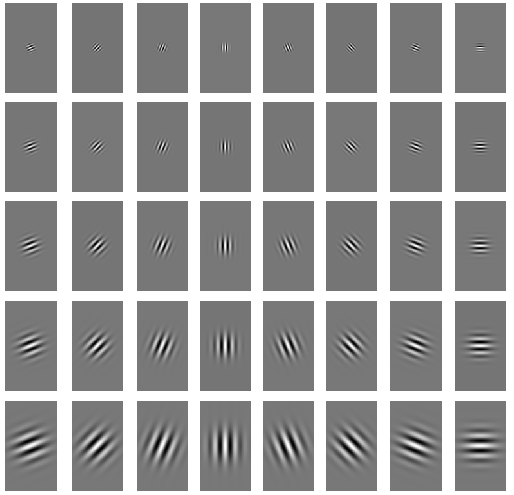
\includegraphics[height=6cm]{gabor-orientations.png}

        \caption{The real part of a Gabor function for five different scales and eight different orientations.}
        \label{fig:gabor-orientations}
    \end{subfigure}
    \caption[\url{http://www.intechopen.com/source/html/16592/media/image74.png}]{Detailed feature filters}
\end{figure}
    
Itti et al. (2001) refines Koch's findings and describes the early stages more in detail. It explains different strategies for
detection of  features, mostly using center-sourround filters (see Figure~\ref{fig:difference-of-gaussians}) on any kind
of contrast-based feature, derived from color. More interesting are edge detection filters, implemented by \textsc{Gabor
kernels}. These kernels are the product of a center-sourround filter (difference of Gaussians) and a sinusoidal
function. They exists for different sizes and all orientations (Figure~\ref{fig:gabor-orientations}).

Furthermore, the model explains the mechanism for merging the feature maps into a general saliency map. Important in this
process is the weighting of the different features, i.e. how important having a special\footnote{read: different from
the others, high contrast} color is in comparison to having a special orientation. Itti finds that there are two main
factors that impact this weighting -- one being top-down, cognitive decision, the other being training. However, there
seem to be no strong interactions between the different feature maps, such as especially high saliency for a combination
of a specific color with a specific orientation. The ability to detect these combinations can also not be learned, which
leads to the conclusion that the feature weighting is the first stage in the visual system influenced by learning.

\subsection{Perazzi 2012 -- Contrast Based Filtering for Salient Region Detection}

Perazzi et al. try to provide a fast and reliable application-oriented algorithm for salient region detection. This is
different in detecting saliency points in that it tries to retain object features in the saliency map, especially
boundaries of the salient objects. Special about this method is that it is possible to implement with only using
Gaussian blur functions. This is a huge convenience for achieving great performance due to the ability to decompose
multidimensional blurs into multiple passes.

The Perazzi model first decomposes the input image into segments, using an edge-preserving algorithm. It uses a variation of
SLIC, a simple K-means clustering algorithm using geodesic image distance in Lab color space. The yielded segments,
called \emph{elements}, are then analysed for uniqueness and distribution.

Uniqueness denotes the rarity of the element color, compared to all other
segments, weighted by the distance between them. By choosing a constant weight
function independent of the distance, the global uniqueness is determined, while
a local weight function may overemphasize object boundaries. Perazzi et al. therefor choose
a Gaussian function for the weight and show that this gives good, not-too-
localized results and is decomposable by axis.

The second feature, distribution, measures the occurence of a color elsewhere in the image. A low variance indicates a
compact object, which in the Perazzi model is considered more salient. A very similar Gaussian weight function is used, such that the
position needs to be blurred in color space, again being decomposable by color component axis. After calculating both
features for each element, the elements are assigned a saliency from the features, which are then applied to the
original image pixels by an up-sampling algorithm.

\subsection{Hou 2007 -- Saliency Detection: A Spectral Residual Approach}

Hou found that in natural scene images, frequency analysis yields a typical average pattern. The difference between the
frequency analysis of a specific image to this average pattern returns what spatial frequencies in the image are \emph{special},
that is, are not just average image data but some kind of interesting object. From these frequencies, the original
places in the image can be looked up in reverse, producing a saliency map.

This model is independent of low-level features, but rather works by detecting what parts of the image are not ``background
noise''. The great advantage of this is the generality of the system. There are however no findings that similar processes are
going on in the human brain, so this model is -- similar to the Perazzi model -- just a technical solution for the visual
attention tasks performed by the brain.

\section{Discussion}

\subsection{Algorithm Requirements}

In this section I will compare the algorithms and methods and explain in detail which features may be relevant for
specific kinds of task, and how they are introduced.

When comparing saliency maps produced by different state-of-the-art methods, one immediately finds a huge difference in
the \emph{blurriness} of the object. This is usually a result of center-sourround filters, as they work by taking
neighboured pixels (stimuli) into account. In practical examples, more blurriness is often introduced when the image is
downsampled, since many local contrast functions have complexity $\mathcal{O}(n^2)$, and downsampling greatly reduces
the number of pixels.

While blurriness is not a problem in finding single points of interest (winner-take-all), it does remove detail from the
map. This particularly impedes object detection, as the boundaries cannot be retrieved from the saliency map. This
task is performed in the ventral pathway, and does not require the saliency map. In technical solutions however, it may be
desirable to reduce the amount of work and generalize both pathways into one algorithms.

A second feature desired from an algorithm is the ability to sort the salient points by intensity, to \emph{determine an
order} for the attention flow. This is quite the opposite to boundary detection, which is a binary decision (``part of
the object or not?''). Some algorithms not presented in this paper completely lack this feature by only calculating 
local saliency measures, not taking into account the whole scene (``is there any object even more interesting?'').

Further features of interest are the ability for \emph{iterative saliency analysis}, giving approximate results quickly
and  refining the exact saliency over time, which can be quite useful in the field of robotics, where quick decisions
have to be made, but slower corrections may be desireable.

Also, many algorithms only consider static visual scenes, while spatio-temporal data cannot always be processed. This is
essential for \emph{movement detection} and quite obviously an important task for the human brain.

\subsection{Comparison}

It is easily possible to separate any method into two categories -- neural models and computational models. The
approaches by Itti/Koch and Perazzi are exceedingly good examples for both categories, respectively. While neural models
try to  explain the visual system, they mostly try to emulate the pre-attentive stage. This stage is highly
parallel\cite{itti2001} and only yields the location of salient points. Thus, these models cannot be used selfcontained
and are rather theoretical than practical. Moreover, parallel computations as in neural networks are hard to evaluate
with artificial computational devices, rendering these approaches useless for real-time applications.

The computational models go further, using basic features like the neural models to compute some kind of saliency map
that may already contain sequential-type computations as found in the higher levels of the visual system. While these
are generally  easier to compute, they are often specialized for specific tasks and do not provide the great reliability
of the visual system.

Table~\ref{tbl:comparison} compares the categories according to above-mentioned desired features using the exemplary
approaches by Itti/Koch, Perazzi and Hou.

\begin{table}[hbt]
    \scriptsize
    {
    \def\arraystretch{1.5}
    \begin{tabularx}{\textwidth}{lXXX}
    \hline
    \textbf{Approach}
        & \textbf{Itti/Koch} 
        & \textbf{Perazzi}
        & \textbf{Hou} \\ 
    \hline
    Model type
        & neural
        & computational
        & computational \\
    Figure~\ref{fig:examples} column
        & (b)
        & (g)
        & (c) \\
    \hline
    Object detection     
        & impossible              
        & great (with contours)
        & good \\
    Order of interest     
        & good / inhibition of return              
        & fair
        & fair \\
    Iterative analysis  
        & simple
        & not possible
        & n/a \\
    Movement detection      
        & use 3-dim. input space
        & possible
        & difficult \\
    \hline
    \end{tabularx}
    }

    \caption{Comparison between approaches and their features and capabilities}
    \label{tbl:comparison}
\end{table}

\newpage
\section{Conclusion}

I have found that there exists a great variety of saliency detection methods for a wide area of applications. However,
each method is specialized for different features, with only very few focusing on being a general model.

The most referenced and most neuro-biologically plausible model was defined by Itti/Koch. This model explains the workings
of the human brain and can easily be implemented using neural structures. However, it returns very blurred saliency maps
that are not useful in every context.

More computationally oriented approaches like Perazzi and Hou were derived from the works of Koch and Itti in recent years,
however, while being easier to implement using computer hardware, these approaches are often more task specific and
less biologically founded.

Overall, saliency detection is a field of research in neuroinformatics that did receive and still receives lots of
attention. I has great potential for it has many possible use cases throughout science and industry.

% APPENDIX %

\newpage
\nocite{*}
\bibliographystyle{plain}
\bibliography{sources}

\listoffigures

\listoftables

\end{document}